\section*{Part C}
\addcontentsline{toc}{section}{Part C}

\lstinputlisting[
  caption = Requirement (a) MATLAB code,
  label = code:C_r_a,
]{matlab/C_r_a.m}

\begin{figure}[htbp]
  \centering
  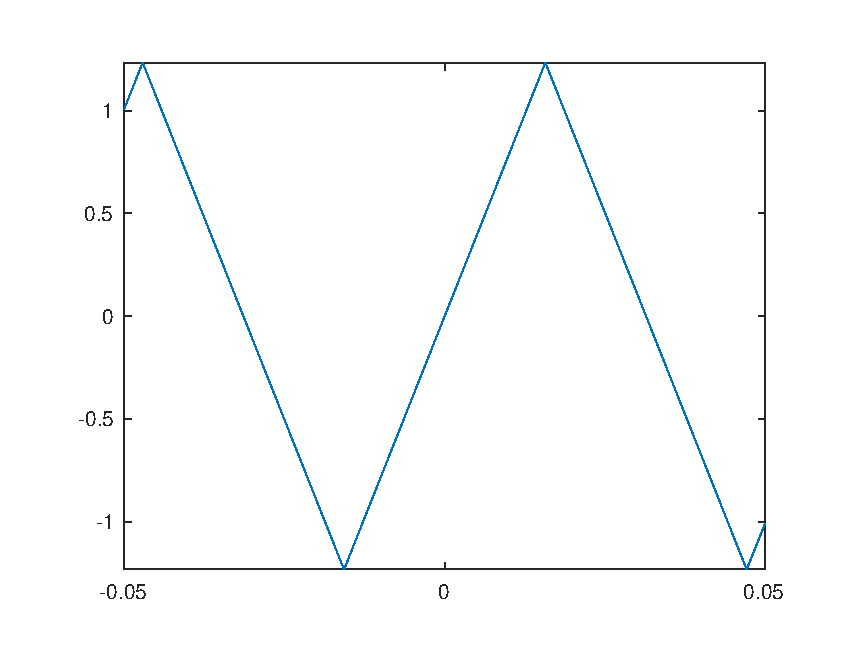
\includegraphics [width=3.7in]{matlab/fig/C_r_a.eps}
  \caption{waveform of $f_1(t)=\sin\omega_o t - \frac{1}{9}\sin3\omega_o t + \frac{1}{25}\sin5\omega_o t - \frac{1}{49}\sin7\omega_o t + \dots$}    
  \label{fig:C_r_a}
\end{figure}

This is a triangular wave. It consists only of sin components, so it is rightly an odd function. Its absolute peak values are slightly larger than 1.

\lstinputlisting[
  caption = Requirement (b) MATLAB code,
  label = code:C_r_b,
]{matlab/C_r_b.m}

\begin{figure}[htbp]
  \centering
  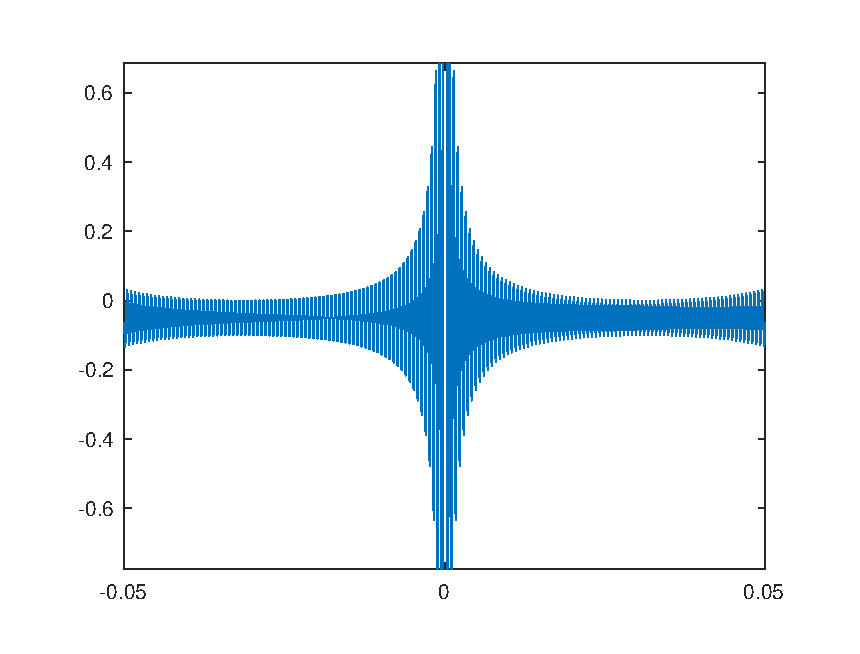
\includegraphics [width=4in]{matlab/fig/C_r_b.eps}
  \caption{waveform of $f_2(t)=0.1(\cos\omega_o t + \cos2\omega_o t + \cos3\omega_o t + \cos4\omega_o t + \dots)$}    
  \label{fig:C_r_b}
\end{figure}

This signal has infinite values around 0. At both ends, it stays in the same interval of undulation.

\lstinputlisting[
  caption = Requirement (c) MATLAB code,
  label = code:C_r_c,
]{matlab/C_r_c.m}

\begin{figure}[htbp]
  \centering
  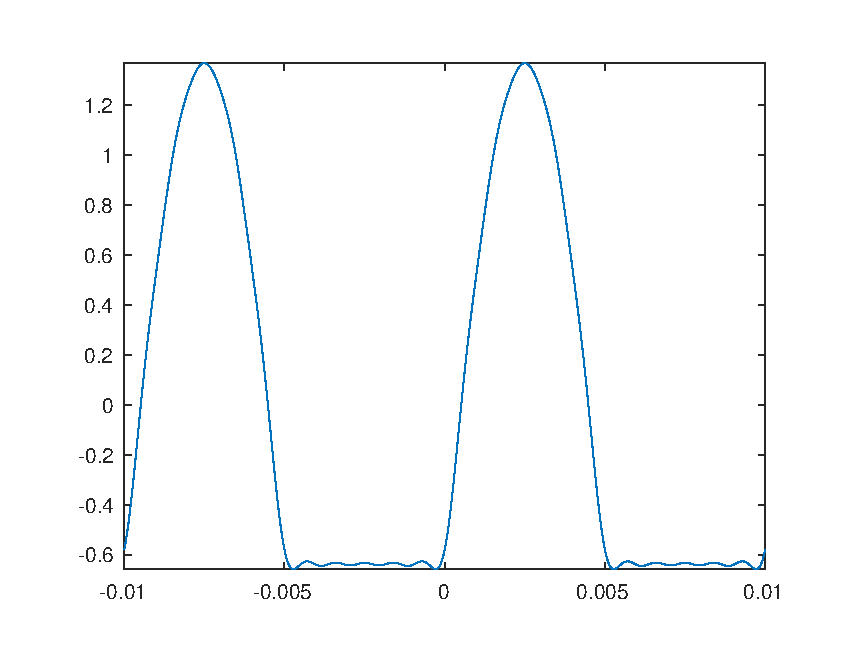
\includegraphics [width=4in]{matlab/fig/C_r_c.eps}
  \caption{waveform of $f_3(t)=\sin\omega_o t - \frac{4}{3\pi}\cos2\omega_o t - \frac{4}{15\pi}\cos4\omega_o t - \frac{4}{35\pi}\cos6\omega_o t - \frac{4}{63\pi}\cos8\omega_o t - \frac{4}{99\pi}\cos10\omega_o t$}    
  \label{fig:C_r_c}
\end{figure}

The bottom of this signal is like a broken straight line and the top is like a sinusoidal wave. The bottom is as if it has been cut off. The waveform is neither axisymmetric nor centrosymmetric. This can also be inferred from the fact that its expression contains both sin and cos components.

\lstinputlisting[
  caption = Requirement (d) MATLAB code,
  label = code:C_r_d,
]{matlab/C_r_d.m}

\begin{figure}[htbp]
  \centering
  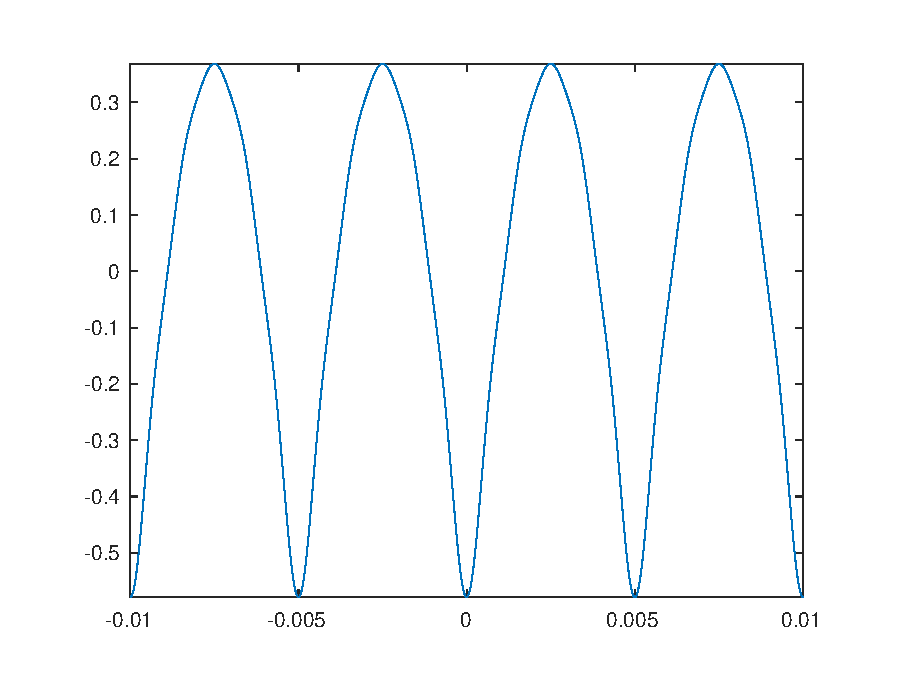
\includegraphics [width=4in]{matlab/fig/C_r_d.eps}
  \caption{$f_3(t)$ without its fundemental component $\sin\omega_o t$}    
  \label{fig:C_r_d}
\end{figure}

When the sin component was removed, only the cos part of the signal remains, so it is logical that it becomes an even function. At the same time, the lower part, which appears to be cut off in Figure \ref{fig:C_r_c}, takes on a sine wave-like form. However, the top of the signal is slightly expanded, while the bottom is slightly contracted.

\pagebreak